% !TEX encoding = UTF-8
% !TEX program = pdflatex
% !TEX root = InformationRetrieval.tex
% !TEX spellcheck = it-IT

% 7 Ottobre 2016

%section indicizzazione

\subsubsection{Vengono sempre eseguite tutte le fasi?}

Non devono essere necessariamente eseguite tutte le fasi, perché ogni fase porta un costo aggiuntivo e non sempre porta un effettivo miglioramento.

\subsection{Fasi del processo di indicizzazione}

Come set di documenti di riferimento utilizziamo i seguenti documenti:

\begin{itemize}
	\item \textbf{D1}: L’enorme quantità di informazioni presenti nelle pagine Web rende necessario l’uso di strumenti automatici per il recupero di informazioni
	\item \textbf{D2}: I presenti hanno descritto le fasi del recupero dell’enorme relitto ma le informazioni non concordano su tipo e quantità di strumenti in uso
	\item \textbf{D3}: \`E stato presentato nel Web un documento che informa sulle enormi difficoltà che incontra chi usa uno strumento informativo automatico
\end{itemize}

Trattandosi di documenti in lingua italiana c'è da prendere in considerazione le lettere accentate e gli apostrofi, inoltre, per evitare ulteriori complicazioni è stata rimossa la punteggiatura.

Si può notare anche la presenza di lettere maiuscole all'interno della frase, che possono essere utilizzate per discriminare i nomi propri.

\begin{figure}[htbp]
\centering
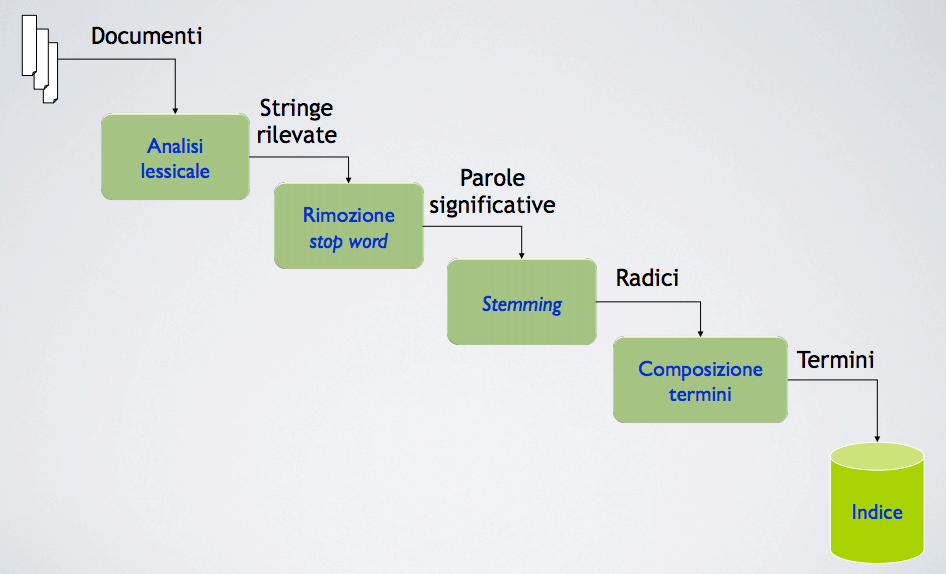
\includegraphics[width=0.7\textwidth]{images/l4-fasi}
\caption{Fasi del processo di indicizzazione. Vengono applicate sia ai documenti che alle query effettuate dall'utente.}
\end{figure}

\subsubsection{Fase 1: Analisi lessicale}

Viene fatta la scansione dei documenti al fine di estrarre dei \textbf{token}, delle parole che sono potenziali descrittori del documento.

I token vengono individuati nel testo tramite dei caratteri di separazione come lo spazio, la tabulazione, ecc. In base alla collezione di documenti può anche essere utile considerare altri caratteri di separazione, come i simboli matematici, le date, ecc.

La gestione delle date, specialmente se queste sono rilevanti, risulta essere molto complicata perché esistono vari formati più o meno compatti per esprimerle.

Ovviamente l'analisi lessicale dipende fortemente dalla lingua, perché per essere efficace deve tenere in considerazione le regole grammaticali.

Nella produzione dei token bisogna tenere conto che questi \textbf{vengono ordinati in ordine alfabetico} e che il più delle volte le parole hanno un significato diverso in base all'ordine in cui sono state scritte. 
Si può quindi scegliere di sacrificare alcune informazioni e tenere l'ordine lessicografico oppure si può fare un'analisi più complessa e tenere traccia anche dell'ordine dei token.

\paragraph{Documenti dopo l'analisi lessicale} La lista dei token ordinata in ordine lessicografico dei documenti di riferimento è:

\begin{itemize}
	\item \textbf{D1}: automatici di di di enorme il informazioni
	informazioni l' l' necessario nelle pagine per presenti quantità recupero rende strumenti uso web
	\item \textbf{D2}:: concordano del dell' descritto di e enorme fasi hanno i in informazioni le le ma non presenti quantità recupero relitto strumenti su tipo uso 
	\item \textbf{D3}: automatico che che chi difficoltà documento è enormi informa informativo incontra nel presentato sulle stato strumento un uno usa web 
\end{itemize}

\paragraph{Alcune problematiche}

I caratteri del documento possono essere codificati in vario modo e possono richiedere più byte per essere rappresentati. 
Questo problema si ripercuote poi sul come leggere il documento, se considerarlo come uno stream di byte o di caratteri.

Rimangono poi i problemi legati alla lingua, che può avere delle notazioni particolari per gli accenti, numeri, date, maiuscole, ecc.

Infine ci sono tutte le problematiche legate all'implementazione, quindi tipi di dato, buffer, memoria impiegata, ecc.

\subsubsection{Fase 2: Rimozione delle stop word} 

Le parole funzionali sono le parole che non portano informazioni ma servono per rendere comprensibili le frasi. Si tratta quindi di articoli, pronomi personali, preposizioni e congiunzioni.
Queste parole vengono anche dette \textbf{stop word}, perché quando vengono incontrate è necessario fermarsi e decidere se tenerle o meno.

Nel caso di collezioni di documenti specifici possono essere considerate come stop word anche delle parole comuni per quel determinato argomento.

Per il caso generale sono disponibili delle \textbf{stop list} pre-compilate che contengono le stop word tipiche per una determinata lingua e che vengono redatte da dei linguisti.

Tipicamente conviene rimuovere le stopword perché così facendo diminuisce notevolmente la dimensione dell'indice, questo perché sono poche parole ma molto frequenti.

Una possibile lista di stop word per i nostri documenti è data da:

\begin{center}
	\textit{che chi del dell’ di e è hanno i il in l’ le ma nel
		nelle non per stato su sulle un uno }
\end{center}

Da notare che nella lista compaiono anche l'ausiliare ``è'' e il sostantivo ``stato''.

\paragraph{Documenti dopo la rimozione delle stop word} Una volta rimosse le stop word il risultato è:

\begin{itemize}
	\item \textbf{D1}: automatici enorme informazioni informazioni necessario pagine presenti quantità recupero rende strumenti uso web 
	\item \textbf{D2}: concordano descritto enorme fasi informazioni presenti quantità recupero relitto strumenti tipo uso
	\item \textbf{D3}: automatico difficoltà documento enormi incontra informa informativo presentato strumento usa web
\end{itemize}

\paragraph{Problematiche della rimozione}

Rimuovere le parole riduce pesantemente la dimensione dell'indice, ma questo richiede di avere a disposizione una stop list per ogni lingua con cui si vuole lavorare e la ricerca all'interno della lista deve essere fatta in modo efficiente.

C'è però un problema perché dall'indice non si riesce più a ricostruire la semantica della frase di partenza. Una possibile soluzione è di tenere una copia dell'elenco che contiene anche le stopword, sennò se questo non è possibile si può ridurre al minimo il numero di stop word da eliminare.

\subsubsection{Fase 3: Stemming}

Lo \textbf{stemming} o \textbf{conflation} è una fase dell'indicizzazione in cui vengono gestite le forme varianti di una parola, come le forme singolare/plurale oppure tutte quelle parole che hanno una radice in comune.

Lo specifico obiettivo è quello di ridurre le forme differenti di una parola ad una radice semantica comune al fine di ridurre la dimensione dell'indice.

Anche in questo caso gli algoritmi dipendono dalla lingua e possono essere sviluppati sia in modo statistico che in modo linguistico.

L'algoritmo che esegue lo stemming viene chiamato \textbf{stemmer} e può essere implementato con due apprcci:

\begin{itemize}
	\item \textbf{Algoritmico}: viene utilizzato un programma per decidere se due parole sono collegate. Spesso si basa sulla conoscenza dei suffissi di una specifica lingua.
	\item \textbf{Dictionary based}: vengono utilizzati uno o più dizionari, preparati in precedenza e che mantengono le relazioni esistenti tra i vari termini.
\end{itemize}

Lo stemmer prende il nome di \textbf{suffix-stemmer} quando riduce le parole inglesi dalla forma plurale a quella singolare, rimuovendo solamente la \textit{s} finale. Bisogna però stare attenti ai plurali irregolari come ``\textit{centuries}'' o ad alcuni casi in cui i termini non sono plurali anche se finiscono per \textit{s} come ``\textit{is}''. Il suffix-stemmer più famoso è quello di Porter (1980).

\paragraph{Effetti dello stemming}

Lo stemming è un processo intuitivo e che permette di ampliare il automaticamente il range dell'interrogazione effettuata dall'utente, perché viene applicato anche alla query. A volte questo effetto può essere desiderato, altre volte no, ma tipicamente è preferibile fornire più documenti per un discorso di frustrazione dell'utente.

Ci sono però dei casi in cui lo stemming crea confusione, ad esempio con i termini ``\textit{dentellato}'' e ``\textit{dentifricio}'' perché hanno la stessa radice ma hanno un significato diverso.

\paragraph{Documenti dopo lo stemming}
Sono rimaste 20 radici distinte, ma il contenuto dei documenti è quasi impossibile da capire.

\begin{itemize}
	\item \textbf{D1}: autom enorm inform inform necessar pagin present quantit recuper rend strument us web
	\item \textbf{D2}: concord descr enorm fas inform present quantit recuper relitt strument tip us
	\item \textbf{D3}: autom diffic document enorm incontr inform inform present strument us web
\end{itemize}

Volendo si può scegliere di tenere più di un'indice, uno in cui viene fatto lo stemming e uno in cui non viene fatto o viene fatto in modo più leggero. Così facendo si può scegliere quale dei due utilizzare in base all'utente, tanto al giorno d'oggi non ci sono problemi di memoria secondaria.

\paragraph{Problemi dello stemming}

Come già detto serve uno stemmer per ogni lingua e in ogni caso è difficile riconoscere tutte le forme irregolari.

Possono inoltre verificarsi delle situazioni di \textbf{over-stemming} e \textbf{under-stemming}, ovvero quando il risultato finale è troppo corto (ho tagliato troppo) o troppo lungo (ho tagliato troppo poco).













